\documentclass{article}
\usepackage{tikz}
\usepackage{CJKutf8}
\usepackage{amsmath}
\usepackage{amsthm}
\begin{document}
\begin{CJK}{UTF8}{gbsn}
\newtheorem{Exercise}{习题}

\begin{Exercise}
  设$G$为一个有$p$个顶点的图,$\delta(G) \geq (p+k-2)/2$,$p\geq 2$,试证:$G$为$k$-连通的,其中$k<p$。
\end{Exercise}
\begin{proof}[证明]
  设$G'$为$G$去掉任意的$k-1$个顶点所得到的一个图,以下证明$G'$为连通的。用反证法,假设$G'$不连通,则至少有一个支$G_1$,其顶点数小于等于$\frac{p-(k-1)}{2}$。
  设$v$为$G_1$中的任意一个顶点,则$v$在$G$中的度
  \[\deg v \leq \frac{p-(k-1)}{2} - 1 + (k-1) = \frac{p+k-3}{2}\]
矛盾。
\end{proof}
\begin{Exercise}
  设$G$为一个三次正则图,试证:$\kappa(G)=\lambda(G)$
\end{Exercise}
\begin{proof}[证明]
  (1)如果$\kappa(G)=0$,则$G$不连通,此时$\lambda(G)=0$,故$\kappa(G) = \lambda(G)$。

(2)如果$\kappa(G)=1$,则$G$中存在顶点$u$,$G-u$不连通。由$\deg u=3$知,$G-u$至少存在一个分支只有一条边与$u$相连,显然去掉这条边之后,$G$不连通,所以$\lambda(G)=1$,故$\kappa(G)=\lambda(G)$。

(3)如果$\kappa(G)=2$,则存在两个顶点$v_1$和$v_2$,$G-\{v_1,v_2\}$不连通。$G-v_1$是连通的,且$G-v_1-v_2$不连通,类似于(2)中的讨论知$G-v_1$中存在一条边$e_2$,$G-v_1-e_2$不连通。另一方面由$\lambda(G)\geq \kappa(G)=2$知$G-e_2$是连通的,由于$G-e_2-v_1=G-v_1-e_2$不连通,由与(2)类似的讨论知$G-e_2$中存在一条边$e_1$,$G-e_2-e_1$不连通,所以$\lambda(G)=2$,故$\kappa(G)=\lambda(G)$。

(4)如果$\kappa(G)\geq 3$,由$\kappa(G) \leq \lambda(G) \leq \delta(G) = 3$知,$\kappa(G)=\lambda(G)=3$。
\end{proof}
\begin{Exercise}
  设$r\geq 2$,$G$是$r$正则图且$\kappa (G)=1$。证明:$\lambda(G) \leq [\frac{r}{2}]$。
\end{Exercise}
\begin{proof}[证明]
  因为$\kappa(G)=1$,所以$G$有一个割点$v$。由$\deg v = r$,且$G-v$有至少两个分支知,存在一个分支,$v$与该分支的顶点联结的边数小于等于$[\frac{r}{2}]$,去掉这些边,$G$不连通,从而$\lambda(G) \leq [\frac{r}{2}]$。
\end{proof}
\begin{Exercise}
  构造一个图$G$,使得$\kappa(G)=3,\lambda(G)=4,\delta(G)=5$。
\end{Exercise}
\begin{proof}[解]
\mbox{} \par \noindent

 \begin{center} 
  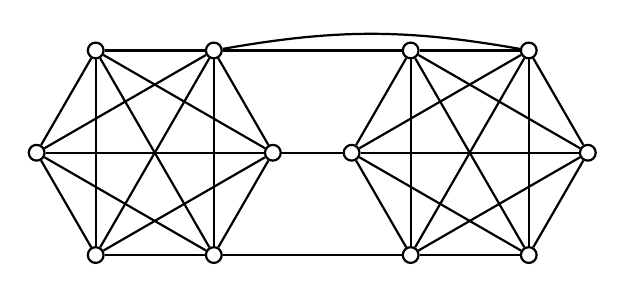
\begin{tikzpicture}[auto,
    specification/.style ={circle, draw, thick, inner sep = 0pt, minimum size=2mm}]
   \node[specification] (A)  at (0:1.5cm)  {};
   \node[specification] (B)  at (60:1.5cm)  {};
   \node[specification] (C)  at (120:1.5cm)  {};
   \node[specification] (D) at (180:1.5cm)  {};
   \node[specification] (E)  at (240:1.5cm)  {};
   \node[specification] (F)  at (300:1.5cm)  {};

   \node[specification] (G)  at ([xshift=4cm]0:1.5cm)  {};
   \node[specification] (H)  at ([xshift=4cm]60:1.5cm)  {};
   \node[specification] (I)  at ([xshift=4cm]120:1.5cm)  {};
   \node[specification] (J) at ([xshift=4cm]180:1.5cm)  {};
   \node[specification] (K)  at ([xshift=4cm]240:1.5cm)  {};
   \node[specification] (L)  at ([xshift=4cm]300:1.5cm)  {};

   
   \draw[thick] (A) to  (B);
   \draw[thick] (A) to  (C); 
   \draw[thick] (A) to  (D);
   \draw[thick] (A) to  (E);
  
   \draw[thick] (B) to  (C);
   \draw[thick] (B) to  (D);
   \draw[thick] (B) to  (E);
   \draw[thick] (B) to  (F);
  
   \draw[thick] (C) to  (D);
   \draw[thick] (C) to  (E);
   \draw[thick] (C) to  (F);
   


   \draw[thick] (D) to  (E);
   \draw[thick] (D) to  (F);
   \draw[thick] (E) to  (F);
   \draw[thick] (F) to  (A);

   \draw[thick] (G) to  (H);
   \draw[thick] (G) to  (I);
   \draw[thick] (G) to  (J);
   \draw[thick] (G) to  (K);


   
   \draw[thick] (H) to  (I);
   \draw[thick] (H) to  (J);
   \draw[thick] (H) to  (K);
   \draw[thick] (H) to  (L);
   
   \draw[thick] (I) to  (J);
   \draw[thick] (I) to  (K);
   \draw[thick] (I) to  (L);
   


   \draw[thick] (J) to  (K);
   \draw[thick] (J) to  (L);
   
   \draw[thick] (K) to  (L);

   \draw[thick] (L) to  (G);

   \draw[thick] (A) to  (J);
   \draw[thick] (F) to  (K);
   \draw[thick] (B) to  (I);
   \draw[thick] (B) to [bend left = 10] (H);
 \end{tikzpicture}
\end{center}
  
\end{proof}

  \begin{Exercise}
    证明:图$G$为2-边连通的当且仅当$G$的任意两个不同的顶点间有两条边不相交路。
  \end{Exercise}
  \begin{proof}[证明]
    设$x$为$G$的任意一条边,其两个端点为$u$和$v$,由已知条件,$u$和$v$之间有两条边不相交路,去掉边$x$,$u$和$v$之间至少还有一条路,从而$G-x$连通,即图$G$为2-边连通的。
    
    设$G$为2-边连通的,$u$和$v$为$G$的两个不同的顶点,以下施归纳于$u$与$v$之间的距离$d(u,v)$来证明$u$与$v$之间有两条边不相交路。当$d(u,v)=1$时,由于$\lambda(G)\geq 2$,所以$G-uv$连通,在$G-uv$中$u$与$v$之间还有一条路,所以$u$与$v$在$G$中有两条边不相交路。设对于$G$中的任意两个顶点$u$和$v$,当$d(u,v)=k$时,$u$与$v$之间有两条边不相交路。以下证明对于$G$中的任意两个顶点$u$和$v$,当$d(u,v)=k+1$时, $u$与$v$之间有两条边不相交路。由$d(u,v)=k+1$知$u$与$v$之间有一条长为$k+1$的路$P:uv_1v_2\cdots v_kv$。显然$d(u,v_k)=k$。由归纳假设,$u$与$v_k$之间有两条边不相交路$Q$和$W$。由于$\lambda(G)\geq 2$,所以$G-v_kv$为连通图。于是,$G-v_kv$中存在从$u$到$v$的路$S$。$u$为$Q,W,S$的公共顶点。设$w$为$S$上从$u$到$v$且在$Q$或$W$上的最后一个顶点。不妨设$w$在$Q$上,则在$G$中$u$和$v$之间存在两条边不相交路:$Q$上的$u$与$w$间一段后接$S$上$w$与$v$间的那一段所构成的一条路,$W$后接$v_kv$所构成的另一条路。

  \begin{center} 
  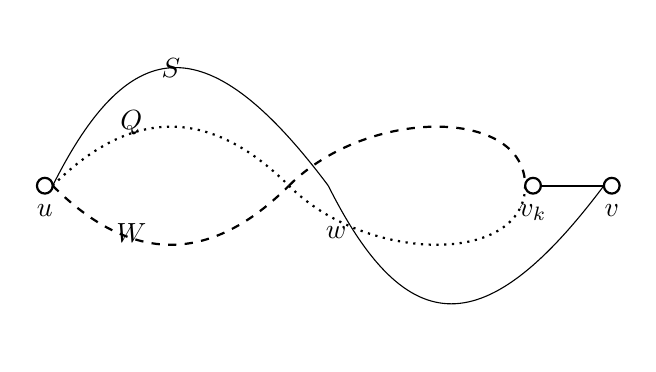
\begin{tikzpicture}[auto,
    specification/.style ={circle, draw, thick, inner sep = 0pt, minimum size=2mm}]
   \node[specification] (A) [label=270:$u$] at (-0.1,0)  {};
   \node[specification] (B) [label=270:$v_k$] at (6.1,0)  {};
   \node[specification] (C) [label=270:$v$]at (7.1, 0) {};

      \draw (1.5,1.5) node {$S$};

   \draw (1,0.8) node {$Q$};
   \draw (1,-0.6) node {$W$};

      \draw (3.6,-0.6) node {$w$};

   
    \draw[thick] (B) to  (C);

   \draw[dotted,thick] (0,0) ..  controls (1,1) and (2,1) .. (3,0);
   \draw[dotted,thick] (3,0) .. controls (4,-1) and (6,-1) .. (6,0);

   \draw[dashed,thick] (0,0) ..  controls (1,-1) and (2,-1) .. (3,0);
   \draw[dashed,thick] (3,0) .. controls (4,1) and (6,1) .. (6,0);

   \draw (0,0)  .. controls (1,2) and (2,2) .. (3.5, 0);
   \draw (3.5,0)  .. controls (4.5,-2) and (5.5,-2) .. (7, 0);

 \end{tikzpicture}
\end{center}

  \end{proof}

\end{CJK}
\end{document}


%%% Local Variables:
%%% mode: latex
%%% TeX-master: t
%%% End:
